% !TEX root = main.tex
% Main text: abstract through conclusion. Proofs are in the appendix; numerical checks in Paper2/checks/.
\begin{abstract}
Two training distributions can agree on every local statistic, every Bayes predictor and, up to a vanishing total-variation distance, on everything else,
yet make gradient training of the same attention model polynomially slower. We prove this for a one-block attention--ReLU Transformer whose
reduced dynamics are derived from its matrices. The mechanism is credit cancellation: attention reads every prefix position, so correlations of order
$\tfrac{1}{N}$ between the source and the other positions, invisible one at a time, add up and cancel the gradient credit reaching the rule.
With independent context the routing time is $\Theta(N\log(1+\varepsilon^{-2}))$ from initialization scale $\varepsilon$; with cancelled credit it is $\Theta(\tfrac{N}{\varepsilon})$,
and over-cancellation stops learning entirely below an exact initialization barrier. The cancellation can be made distributional, so that no function
of what uniform attention reads carries rule credit; a single earlier step that displays the negation of the current state suffices.
Corrupted chain-of-thought supervision is our motivating case: a causal error process with a constant fraction of wrong steps produces the delay at every supervised position,
while independent errors only rescale time by $\tfrac{1}{1-2\eta}$.
The bottleneck is fragile in a useful way: mixing a fraction $\lambda$ of traces without cancellation gives routing time
$\Theta\bigl(N\min\{\tfrac{1}{\varepsilon},\tfrac{1+\log(1+\lambda/\varepsilon)}{\lambda}\}\bigr)$, so $\lambda$ of the order of $\varepsilon$ already removes it.
Beyond the four-scalar model, we prove that when every matrix entry trains under cross-entropy, the cancelled law keeps the network
within distance $\varepsilon$ of its structured initialization, with loss above $\log2-O(\varepsilon^3)$, for time $\Omega(\tfrac{1}{\varepsilon})$.
Exact population experiments check every rate. From fully random initialization the laws separate in reliability rather than speed:
with Adam, every run on the independent law reaches the Bayes predictor, while about a third to a half of runs on the cancelled laws stall at the same sub-optimal stationary point.
\end{abstract}

% ===================================================================
\section{Introduction}
\label{sec:intro}

When can two data distributions that look the same to every local test train a network at very different speeds?
We give an exact answer for attention. An attention head that must learn where to look reads all $N$ prefix positions at once.
If each of them correlates with the target-relevant position by only $-\tfrac{1}{N-1}$, no single statistic notices, but their sum cancels the
gradient credit that would teach the network its rule. The network then sits near its initialization for a time of order $\tfrac{1}{\varepsilon}$
instead of $\log\tfrac{1}{\varepsilon}$.

\paragraph{A saddle made by the data.}
Slow escape from small initialization is familiar from deep linear networks, where a product of small factors creates a saddle
\citep{saxe2014exact,shamir2019exponential}. The saddle here has a different origin. Our model has the same depth under both laws and the same
source--target correlation; what differs is how the other positions correlate with the source. The cancellation turns the linear growth of a
conserved primitive into quadratic growth, and that changes the escape time from logarithmic to inverse in $\varepsilon$.
Weak-gradient analyses \citep{shalevshwartz2017failures,abbe2025parities} relate slow learning to weak target correlation; here the target correlation is fixed
and only the sum over attended positions cancels.

\paragraph{Corrupted chain-of-thought as the motivating case.}
Reasoning traces used for supervision can contain incorrect intermediate steps \citep{havrilla2024noise,zhou2024noisyrationales},
and a model can still learn the correct rule when it remains the most likely next step \citep{natarajan2013noisy,patrini2017loss}.
For modulo-two counting the clean step is $x_{i+1}=b_{i+1}x_i$; a corrupted trace shows $x_{i+1}=b_{i+1}x_i\xi_{i+1}$ with $\Pr(\xi_{i+1}=-1)=\eta$.
At uniform attention the rule gradient factorizes into reliability and contextual credit:
\[
 -\pd{\mathcal L}{r_1}
 =\frac{r_2}{2N}
 \underbrace{(1-2\eta)}_{\text{label reliability }\gamma}
 \underbrace{\left(1+\sum_{j=1}^{N-1}\E[x_Nx_j]\right)}_{\text{contextual credit }\kappa}.
\]
Independent errors lower $\gamma$, which only rescales time. Errors that make earlier steps anti-correlate with the current state lower $\kappa$,
which changes the order of the routing time. A single earlier step that displays the negation of the current state is enough.
Such steps arise when slips are more frequent where the correct state agrees with most earlier steps, so that wrong steps keep the displayed
history balanced; \cref{thm:causal} shows that this error process produces exact cancellation at every supervised step.

\begin{figure}[t]
\centering
\resizebox{\linewidth}{!}{% Conceptual figure: what uniform attention reads under the two matched laws.
\begin{tikzpicture}[>=Stealth, font=\small,
  src/.style={rectangle, rounded corners=2pt, draw=royalazure!80!black, fill=royalazure!14, minimum width=9mm, minimum height=6mm, inner sep=1pt},
  dec/.style={rectangle, rounded corners=2pt, draw=black!45, fill=black!5, minimum width=9mm, minimum height=6mm, inner sep=1pt},
  anti/.style={rectangle, rounded corners=2pt, draw=red!70!black, fill=red!10, minimum width=9mm, minimum height=6mm, inner sep=1pt},
  qry/.style={rectangle, rounded corners=2pt, draw=orange!80!black, fill=orange!14, minimum width=9mm, minimum height=6mm, inner sep=1pt}]

% (a) independent decoys
\begin{scope}
  \node[font=\small\bfseries, anchor=west] at (-0.2,2.25) {(a) independent law $\mathcal D_1$};
  \node[dec] (d1a) at (0,1.2) {$x_1$};
  \node[dec] (d2a) at (1.15,1.2) {$x_2$};
  \node at (2.15,1.2) {$\cdots$};
  \node[dec] (d3a) at (3.15,1.2) {$x_{N-1}$};
  \node[src] (sa) at (4.45,1.2) {$x_N$};
  \node[qry] (qa) at (2.2,-0.55) {$b\ \to\ y$};
  \foreach \d in {d1a,d2a,d3a} { \draw[->, black!45] (\d.south) -- (qa.north); }
  \draw[->, thick, royalazure] (sa.south) -- (qa.north);
  \node[font=\scriptsize, align=center, text=black!70] at (2.2,-1.45)
     {decoys independent of $x_N$:\quad $\E[y b\,x_j]=0$};
  \node[font=\scriptsize, align=center, text=royalazure] at (2.2,-2.05)
     {rule credit at uniform attention $=\frac{\gamma}{N}\cdot 1$};
\end{scope}

% (b) one anti-copy at a random position
\begin{scope}[shift={(7.2,0)}]
  \node[font=\small\bfseries, anchor=west] at (-0.2,2.25) {(b) anti-copy law $\mathcal D_0$};
  \node[dec] (d1b) at (0,1.2) {$x_1$};
  \node[anti] (d2b) at (1.15,1.2) {$-x_N$};
  \node at (2.15,1.2) {$\cdots$};
  \node[dec] (d3b) at (3.15,1.2) {$x_{N-1}$};
  \node[src] (sb) at (4.45,1.2) {$x_N$};
  \node[qry] (qb) at (2.2,-0.55) {$b\ \to\ y$};
  \foreach \d in {d1b,d3b} { \draw[->, black!45] (\d.south) -- (qb.north); }
  \draw[->, red!70!black] (d2b.south) -- (qb.north);
  \draw[->, thick, royalazure] (sb.south) -- (qb.north);
  \node[font=\scriptsize, text=red!70!black] at (1.15,1.75) {random position};
  \node[font=\scriptsize, align=center, text=black!70] at (2.2,-1.45)
     {each decoy: $\E[y b\,x_j]=-\frac{\gamma}{N-1}$;\quad multiset $\{x_j\}$ independent of $x_N$};
  \node[font=\scriptsize, align=center, text=red!70!black] at (2.2,-2.05)
     {rule credit at uniform attention $=\frac{\gamma}{N}\bigl(1-(N-1)\cdot\frac{1}{N-1}\bigr)=0$};
\end{scope}
\end{tikzpicture}
}
\caption{\textbf{Two laws with the same local statistics, read by uniform attention.} The query holds the current letter $b$ and
must predict the displayed successor $y=b x_N \xi$, where $\xi$ is an error independent of everything else. In (a) the prefix
positions are independent of the source. In (b) one prefix position, chosen uniformly at random, displays $-x_N$, so each position
correlates with the source by $-\tfrac{1}{N-1}$. This is too small to change any local statistic, but the $N-1$ positions are read
together and cancel the source's contribution (\cref{lem:credit}); the multiset of displayed values is even independent of $x_N$ (\cref{lem:matched}).}
\label{fig:cancel}
\end{figure}

\paragraph{Contributions.}
\begin{enumerate}[leftmargin=*,itemsep=2pt,topsep=2pt]
\item \textbf{Matched laws, separated training times} (\cref{lem:matched,thm:separation}). Laws with the same error rate, marginals and Bayes predictor,
at total-variation distance $O(N^{-1/2})$, give routing times $\Theta(\tfrac{N}{\gamma}\log(1+\varepsilon^{-2}))$ and $\Theta(\tfrac{N}{\gamma\varepsilon})$ under correlation loss,
with absolute constants. A conserved quantity solves the coupled attention--MLP flow exactly. Over-cancellation has an exact barrier: routing succeeds if and only if
$\varepsilon^2>-F(q_0)$. Cross-entropy keeps both orders for escaping the bottleneck.
\item \textbf{Distributional cancellation} (\cref{lem:matched}). Under the anti-copy law the label is independent of everything uniform attention reads,
so every non-attention parameter of any one-block network sees pure label noise at the start; only routing can break the plateau.
\item \textbf{A dose--response law for clean data} (\cref{cor:dilution}). A fraction $\lambda$ of traces without cancellation gives
$\Theta(\tfrac{N}{\gamma}\min\{\tfrac{1}{\varepsilon},\tfrac{1+\log(1+\lambda/\varepsilon)}{\lambda}\})$: the bottleneck disappears once $\lambda$ exceeds the initialization scale.
\item \textbf{The plateau survives full-matrix training} (\cref{thm:fullmatrix}). With every query, key, value, output, MLP and readout entry trained by
cross-entropy, the cancelled law gives $|\E[Yz]|=O(\varepsilon^3)$ throughout an $\varepsilon$-ball around the structured initialization, and gradient flow needs
time $\Omega(\tfrac{1}{\varepsilon})$ to leave it. The proof uses a loss floor and an energy bound, not an invariant manifold.
\item \textbf{Wrong CoT steps can cause it} (\cref{thm:causal}). A causal error kernel with local error rate $\eta$ and a constant fraction of wrong transitions
produces cancellation at every supervised step, with the correct step still Bayes optimal.
\end{enumerate}

\paragraph{The scope of the claim.} The theorems concern a one-block attention--ReLU network with specified matrix directions and four trained scalars,
derived exactly from its matrices (\cref{prop:realization}); \cref{thm:fullmatrix} lifts the lower bound to full-matrix cross-entropy training near the same initialization,
without the exact rates. The separation is in the initialization scale at fixed $N$; it becomes a separation in $N$ only if
$\varepsilon$ is tied to $N$. Complete cross-entropy routing is verified numerically rather than proved. From fully random initialization the first escape from chance
is limited by the product of small weights and takes the same time under every law; the laws then differ in how often training reaches the Bayes predictor.
In a standard two-layer Transformer the laws train equally fast under AdamW and with LoRA on a pretrained model, and separate only under
plain SGD, in the order of $|\kappa|$ (\cref{app:repro}).

% ===================================================================
\section{Model and corruption laws}
\label{sec:setup}
\paragraph{Notation and prediction task.}
The principal notation is $N$ for prefix length, $\eta$ for the error probability,
$\gamma=1-2\eta$ for reliability, $\varepsilon$ for initialization, and $\kappa$ for cancellation.
Vectors and matrices are bold; $\alpha(q)$ is source attention, $\phi(q)$ is effective credit,
and $F(q)$ is the primitive defining the invariant.
Primes denote differentiation with respect to the displayed scalar argument;
for example, $\phi'(q)$ and $\phi''(q)$ are the first and second credit derivatives.
Time derivatives use Leibniz notation, and parameter gradients use $\nabla$.
For a sequence of displayed signs, write $\bm x_{<i}=(x_1,\ldots,x_{i-1})^\top$.
A single prediction reads $\bm x_{<N+1}$ and a signed instruction $b\in\{-1,1\}$, and predicts $y\in\{-1,1\}$.
The last visible state $x_N$ is the source; positions $j<N$ are decoys.
In modulo-two counting, the clean transition is $y=b x_N$.
We write $\Pr$ for probability, $\E$ for population expectation.
Order statements use $\Theta$ with positive comparison constants.

\begin{definition}[Matched prediction laws]
\label{def:law}
A law of $(\bm x_{<N+1},b,y)$ has error probability $\eta$ if
$\Pr(y\ne b x_N\mid x_N,b)=\eta$; its margin is $\gamma=1-2\eta$.
Two laws are matched when they have the same $\eta$ and the same Bayes predictor given $(\bm x_{<N+1},b)$.
\end{definition}

\begin{definition}[The anti-copy law $\Dlaw{\kappa}$]
\label{def:Dkappa}
Fix $N\ge4$, $\eta\in[0,\tfrac{1}{2})$, $\kappa\in[-1,1]$, and $\rho=\tfrac{1-\kappa}{N-1}$.
Draw the source $x_N$ uniform. Draw the number of anti-copies $M=\lfloor1-\kappa\rfloor+\beta$, where
$\beta\in\{0,1\}$ has $\Pr(\beta=1)=1-\kappa-\lfloor1-\kappa\rfloor$, so that $M\in\{0,1,2\}$ and $\E[M]=1-\kappa$.
Choose $M$ of the $N-1$ decoy positions uniformly at random and set them to $-x_N$; draw the remaining decoys independently and uniformly.
Independently draw $b$ uniform and $\xi\in\{-1,1\}$ with $\Pr(\xi=-1)=\eta$;
set $y=b x_N \xi$ and $\gamma=1-2\eta$.
\end{definition}
Write $\bar w=\tfrac{1}{N-1}\sum_{j<N}x_j$ for the decoy average.
Every displayed sign is uniform, and $\E[x_N x_j]=-\rho$ for each decoy.
Under $\Dlaw{1}$ the source is independent of the decoys; under $\Dlaw{0}$ exactly one decoy is the anti-copy $-x_N$, at a random position;
under $\Dlaw{-1}$ two are. In chain-of-thought terms, the anti-copy is an earlier step that displays the negation of the current state.

\subsection{One-block Transformer and initialization}
\label{sec:architecture}
We use one causal attention head followed by a positionwise, four-unit ReLU MLP, with residual connections and a binary readout.
The theoretical architecture omits layer normalization and dropout. Its query attends to the $N$ preceding state positions;
a fixed type mask excludes the query itself and instruction-only positions. This is a specified one-block Transformer,
with a restricted set of trainable directions. Normalization would change the exact identities below.

\paragraph{Embeddings and attention matrices.}
Let $\bm e_i\in\mathbb R^7$ be standard basis columns and let $\bm0$ denote a zero vector.
The state and query embeddings are
\begin{equation}
 \bm h_j^{(0)}=x_j\bm e_1+\bm e_3+\mathbf1[j=N]\bm e_4+\mathbf1[j<N]\bm e_5,
 \qquad \bm h_q^{(0)}=b\bm e_2+\bm e_3.
 \label{eq:embeddings}
\end{equation}
Here $\mathbf1[\cdot]$ is the indicator of the stated condition.
The one-dimensional query, key and value maps and their output projection are
\begin{equation}
 \begin{gathered}
 \bm w_q=\bm e_3^\top,\qquad
 \bm w_k=q_s\bm e_4^\top+q_d\bm e_5^\top,\qquad
 \bm w_v=\bm e_1^\top,\qquad \bm w_o=\bm e_6,\\
 \bm w_q,\bm w_k,\bm w_v\in\mathbb R^{1\times7},\qquad
 \bm w_o\in\mathbb R^{7\times1}.
 \end{gathered}
 \label{eq:attention-matrices}
\end{equation}
For the $N$ unmasked state positions, define the score vector $\bm q$ and attention vector $\bm\alpha$ by
\begin{equation}
 q_j=(\bm w_q\bm h_q^{(0)})(\bm w_k\bm h_j^{(0)}),\qquad
 \bm\alpha=\softmax(\bm q),\qquad
 \bm h_q=\bm h_q^{(0)}+\bm w_o\sum_{j=1}^N \alpha_j\bm w_v\bm h_j^{(0)}.
 \label{eq:attention-block}
\end{equation}
The query/key dimension is one, so the attention scaling factor is $1$.
The attended value is the scalar $v=\sum_j \alpha_j x_j$; the residual $\bm h_q$ is a vector.

\paragraph{Four-unit MLP matrices.}
Fix $B>0$, let $\bm1_4$ be the four-dimensional all-ones vector, and apply $\relu$ coordinatewise to vector arguments. Set
\begin{equation}
 \begin{gathered}
 \bm w_1=\begin{pmatrix}
 r_1\bm e_6^\top+B\bm e_2^\top\\
 -r_1\bm e_6^\top+B\bm e_2^\top\\
 r_1\bm e_6^\top-B\bm e_2^\top\\
 -r_1\bm e_6^\top-B\bm e_2^\top
 \end{pmatrix},\qquad
 \bm b_1=-B\bm1_4,\\
 \bm w_2=r_2\bm e_7(1,-1,-1,1),\qquad
 \bm w_1\in\mathbb R^{4\times7},\quad
 \bm w_2\in\mathbb R^{7\times4},\quad \bm b_1\in\mathbb R^4,\\
 \bm h'_q=\bm h_q+\bm w_2\relu(\bm w_1\bm h_q+\bm b_1),
 \qquad z=\bm e_7^\top\bm h'_q.
 \end{gathered}
 \label{eq:mlp-matrices}
\end{equation}
\paragraph{Initialization and training.}
Choose $0<\varepsilon\le1$ and fix the gate scale before training so that
\begin{equation}
 B>\sqrt{\varepsilon^2+\log(N-1)+1+e}.
 \label{eq:gate-bound}
\end{equation}
The trainable parameters and their initialization are
\begin{equation}
 \bm\theta=(q_s,q_d,r_1,r_2)^\top\in\mathbb R^4,\qquad
 \bm\theta(0)=(0,0,\varepsilon,\varepsilon)^\top.
 \label{eq:initialization}
\end{equation}
Thus $\bm w_k(0)=\bm0^\top$, every score is zero, $\alpha_j(0)=\tfrac{1}{N}$,
and the two MLP factors both start at $\varepsilon$.
All other directions in \cref{eq:attention-matrices,eq:mlp-matrices} are fixed.
We train these four coordinates by population gradient flow in training time $t$, using either loss:
\begin{equation}
 \mathcal L_{\mathrm{corr}}(\bm\theta)=-\frac{1}{2}\E[y z_{\bm\theta}],\qquad
 \mathcal L_{\mathrm{ce}}(\bm\theta)=\E\bigl[\log(1+e^{-y z_{\bm\theta}})\bigr],\qquad
 \frac{d\bm\theta(t)}{dt}=-\nabla_{\bm\theta}\mathcal L(\bm\theta(t)).
 \label{eq:parameter-flow}
\end{equation}
Gradient flow uses the Euclidean metric on the parameter coordinates.
The tied rows contribute through the chain rule; the entries of the matrices are not independent trainable coordinates.
The positional features identify the candidate source, while its attention weight is learned from uniform initialization.

\begin{proposition}[Exact reduction of the one-block network]
\label{prop:realization}
For $b\in\{-1,1\}$ and $|r_1v|<2B$, the network in \cref{eq:attention-block,eq:mlp-matrices} has logit
\begin{equation}
 z=r_1r_2b v.
 \label{eq:model}
\end{equation}
For either population correlation loss or binary cross-entropy, its gradients with respect to the four trainable scalars
are exactly those of \cref{eq:model}. Since all decoys share one score, the attention read is
$v=\alpha(q)x_N+(1-\alpha(q))\bar w$, where
$q=q_s-q_d$ and $\alpha(q)=\tfrac{e^q}{e^q+N-1}$.
\end{proposition}
The proof in \cref{app:network-proof} has three steps: attention, the MLP identity, and the chain rule.

\paragraph{Routing and prediction.}
Define $q=q_s-q_d$, $\alpha(q)=\tfrac{e^q}{e^q+N-1}$, and $q_1=\log(N-1)$.
The routing time is $\Tr:=\inf\{t\ge0:\alpha(q(t))\ge\tfrac{1}{2}\}$, with $\inf\varnothing=\infty$.
At $q>q_1$ and $r_1r_2>0$, $x_N v\ge2\alpha(q)-1>0$ on every prefix;
therefore $\operatorname{sign}(z)=b x_N$ and prediction attains Bayes accuracy $1-\eta$.
The bound in \cref{eq:gate-bound} makes the matrix reduction valid through $q=q_1+1$ for correlation loss,
and through the cross-entropy escape interval; these claims are proved below.
Correlation loss is unbounded below, so the convergence claim concerns prediction, rather than convergence to a finite loss minimizer.

% ===================================================================
\section{Why credit cancels}
\label{sec:cancel}

\begin{lemma}[Credit cancellation]
\label{lem:credit}
Let a law have clean next-step rule $b x_N$ and reliability $\gamma$, and suppose $\xi:=y b x_N$ is independent of $(\bm x_{<N+1},b)$. For correlation loss at uniform attention, in the model of \cref{eq:model},
\[
 -\pd{\mathcal L}{r_1}=\frac{r_2}{2}\cdot\frac{\gamma\,\kappa}{N},
 \qquad
 \kappa:=1+\sum_{j=1}^{N-1}\E[x_N x_j],
\]
and symmetrically for $r_2$. For $\Dlaw{\kappa}$ the coefficient is the parameter $\kappa$ of \cref{def:Dkappa}; in particular the rule gradient vanishes identically
under $\Dlaw0$, and under $\Dlaw{\kappa}$ with $\kappa<0$ it points away from the rule.
\end{lemma}

The proof separates the source contribution $\tfrac{\gamma}{N}$ from the decoy contributions
$(\tfrac{\gamma}{N})\E[x_N x_j]$. The latter are not fixed by the local prediction law.
For $\Dlaw{\kappa}$ they sum to $-\tfrac{\gamma(1-\kappa)}{N}$, so $\kappa=0$ cancels the source contribution.
The full proof is in \cref{app:credit-proof}.

\begin{lemma}[Matched laws and distributional cancellation]
\label{lem:matched}
For every $\kappa\in[-1,1]$, $\Dlaw{\kappa}$ and $\Dlaw1$ are matched (\cref{def:law}): both have rule $y=b x_N$, error rate $\eta$,
and Bayes predictor given the prefix $\hat y=b x_N$ with accuracy $1-\eta$. Every displayed value has the uniform marginal under both.
With $S_{N-1}$ a sum of $N-1$ independent uniform signs and $\tau_N=\tfrac{\E|S_{N-1}|}{2(N-1)}\le\tfrac{1}{2\sqrt{N-1}}$,
\[
 d_{\mathrm{TV}}(\Dlaw{\kappa},\Dlaw1)=(1-\kappa)\,\tau_N\quad(0\le\kappa\le1),\qquad
 d_{\mathrm{TV}}(\Dlaw{\kappa},\Dlaw1)\le\frac{1-\kappa}{2\sqrt{N-2}}\quad(-1\le\kappa\le1).
\]
Under $\Dlaw0$ the multiset $\{x_1,\ldots,x_N\}$ of displayed values is independent of $x_N$, and $y$ is independent of
$(b,\{x_1,\ldots,x_N\})$. Under $\Dlaw1$, $\E[y b x_N]=\gamma$.
\end{lemma}

The matched laws thus differ by an amount that vanishes with $N$ and that no local or Bayes statistic detects. The rest of the paper
shows that this difference changes the training time by a factor polynomial in $\tfrac{1}{\varepsilon}$.
The independence statement is what the untied experiments need. At uniform attention, the attended vector of any one-block network is
the average of the embeddings, which depends only on the multiset of displayed values once all positions receive the same weight.
Under $\Dlaw0$, the label is then a fair coin given everything the MLP and readout see, so their population gradients are those of
pure label noise; only the attention scores can move the network off this plateau.
The obstruction is informational rather than architectural: no function of $(b,\{x_1,\ldots,x_N\})$, of any width, depth or nonlinearity,
is correlated with $y$, so enlarging the MLP or the readout cannot remove it.
A shared-decoy law cannot do this: if every decoy displays one value $w$, the multiset determines $x_N$.

% ===================================================================
\section{Main optimization result}
\label{sec:dynamics}

Decoys share a score, so the flow depends on the scores only through $q=q_s-q_d$, with
$\alpha(q)=\tfrac{e^q}{e^q+N-1}$. Write
\[
 \phi(q)=(1+\rho)\,\alpha(q)-\rho,\qquad \phi'(q)=(1+\rho)\,\alpha(q)\bigl(1-\alpha(q)\bigr),
\]
so that $\E[y b v]=\gamma\,\phi(q)$ and $\phi(0)=\tfrac{\kappa}{N}$ by \cref{lem:credit}. The loss is $\mathcal L=-\tfrac{\gamma}{2}r_1r_2\phi(q)$.

\begin{lemma}[Gradient-flow invariant]
\label{lem:invariant}
From \cref{eq:initialization}, correlation-loss gradient flow under $\Dlaw{\kappa}$ keeps $r_1=r_2=:r>0$, $q_s+q_d=0$, and satisfies
\[
 \ddt{r}=\frac{\gamma}{2}\,r\,\phi(q),\qquad \ddt{q}=\gamma\,r^2\phi'(q).
\]
The quantity $r^2-F(q)$ is conserved, where
\[
 F(q)=\int_0^q\frac{\phi(v)}{\phi'(v)}\,dv.
\]
Hence $r(t)^2=\varepsilon^2+F(q(t))$, $q$ is nondecreasing, and whenever $\varepsilon^2+F>0$ on $[0,q_1]$ the routing time is
\begin{equation}
 \Tr=\int_0^{q_1}\frac{dv}{\gamma\,\bigl(\varepsilon^2+F(v)\bigr)\,\phi'(v)}.
 \label{eq:time}
\end{equation}
For $\kappa\in\{0,1\}$, the gap $q_1+1$ is reached in finite time, and prediction is Bayes optimal whenever $q_1<q(t)\le q_1+1$.
\end{lemma}
\begin{proof}[Derivation of the invariant]
The network output gives $\mathcal L=-\tfrac{\gamma}{2}r_1r_2\phi(q)$.
Differentiating in the original coordinates yields
\[
 \ddt{r_1}=\frac{\gamma}{2}r_2\phi,\quad
 \ddt{r_2}=\frac{\gamma}{2}r_1\phi,\quad
 \ddt{q_s}=\frac{\gamma}{2}r_1r_2\phi'(q),\quad
 \ddt{q_d}=-\frac{\gamma}{2}r_1r_2\phi'(q).
\]
The initialized symmetries preserve $r_1=r_2=r$ and $q_s=-q_d=\tfrac{q}{2}$.
Thus
\begin{align*}
 \frac{d}{dt}(r^2-F(q))
 &=\gamma r^2\phi-\frac{\phi}{\phi'(q)}\gamma r^2\phi'(q)
 &&\text{(chain rule)},\\
 &=0 &&\text{(cancellation)}.
\end{align*}
Its initial value is $\varepsilon^2$; substitution into $\ddt{q}=\gamma r^2\phi'(q)$ gives \cref{eq:time}.
The factor in the score-gap equation comes from subtracting the two score velocities.
Existence, gate validity and prediction are checked in \cref{app:flow-proof}.
\end{proof}


The invariant reduces routing to one integral. Under independent contexts $F$ grows linearly near zero;
under cancellation it grows quadratically, keeping the rule near initialization for longer.

\begin{mainresult}
\begin{theorem}[Matched laws, separated routing times]
\label{thm:separation}
Consider the network and Euclidean gradient flow in \cref{sec:architecture}, initialized by \cref{eq:initialization}.
Let $N\ge4$, $\eta\in[0,\tfrac{1}{2})$, $\gamma=1-2\eta$, and $0<\varepsilon\le1$.
The laws $\Dlaw{\kappa}$, $\kappa\in[-1,1]$, have the same clean rule, error probability and Bayes predictor,
with $d_{\mathrm{TV}}(\Dlaw{\kappa},\Dlaw1)\le\tfrac{1-\kappa}{2\sqrt{N-2}}$.
\begin{enumerate}[label=(\roman*),leftmargin=*,itemsep=2pt,topsep=2pt]
\item \emph{Independent context, correlation loss.}
$\displaystyle \Tr(\Dlaw1)=\Theta\!\left(\frac{N}{\gamma}\log(1+\varepsilon^{-2})\right)$.
\item \emph{Exact cancellation, correlation loss.}
$\displaystyle \Tr(\Dlaw0)=\Theta\!\left(\frac{N}{\gamma \varepsilon}\right)$.
The comparison constants in (i)--(ii) are absolute. Both flows reach the Bayes predictor on the gate-valid interval beyond routing.
\item \emph{Over-cancellation, correlation loss.}
For $-1\le \kappa<0$, put $q_0=\log(1-\kappa)$. Then
\[
 \Tr<\infty\quad\Longleftrightarrow\quad \varepsilon^2>-F(q_0).
\]
At or below the barrier, routing fails and $r(t)\to0$.
The limiting gap is the first zero of $\varepsilon^2+F$ below $q_0$, or $q_0$ at equality.
\item \emph{Escape, binary cross-entropy.}
For fixed $N,\gamma$ there is an escape gap $q_{\mathrm{esc}}>0$ such that, for sufficiently small $\varepsilon>0$,
the times to reach $q_{\mathrm{esc}}$ satisfy
\[
 \Tr_{\mathrm{esc}}(\Dlaw1)=\Theta\!\left(\log\!\frac{1}{\varepsilon}\right),\qquad
 \Tr_{\mathrm{esc}}(\Dlaw0)=\Theta\!\left(\frac{1}{\varepsilon}\right),
\]
and the matrix reduction stays valid on the way.
Here the constants and escape gap may depend on $N,\gamma$.
\end{enumerate}
\end{theorem}
\end{mainresult}

For fixed $N$ and $\gamma$, the ratio $\tfrac{\Tr(\Dlaw0)}{\Tr(\Dlaw1)}$ is of order $\tfrac{1}{\varepsilon\log(\tfrac{1}{\varepsilon})}$. Both routing times are
linear in $N$: \textbf{the separation is in the initialization scale}, not in the prefix length. It becomes a separation in $N$ only if $\varepsilon$ is tied to $N$;
for example $\varepsilon\propto N^{-\tfrac{1}{2}}$ would give $\Tr(\Dlaw1)\lesssim N\log N$ against $\Tr(\Dlaw0)\gtrsim N^{\tfrac{3}{2}}$, but we do not claim that this coupling
is what standard initializations produce for the four tied scalars.

\begin{remark}[Reliability only rescales time]
\label{rem:rescaling}
Correlation loss is linear in the label, so for a fixed displayed-prefix law and an independent error sign, $\mathcal L_\eta=(1-2\eta)\mathcal L_0$.
The whole trajectory is the noiseless one run at speed $\gamma$, and $T(\eta,\kappa)=\tfrac{T(0,\kappa)}{1-2\eta}$ for every $\kappa$, including infinite times.
Independent errors therefore cost a constant factor; contextual credit changes the order.
\end{remark}

\begin{corollary}[A small clean fraction removes the bottleneck]
\label{cor:dilution}
For $0\le\lambda\le1$, the mixture of a fraction $\lambda$ of $\Dlaw1$ with $1-\lambda$ of $\Dlaw0$ is $\Dlaw\lambda$.
Under correlation loss, for $0<\varepsilon\le1$,
\[
 \Tr(\Dlaw\lambda)=\Theta\!\left(\frac{N}{\gamma}\min\left\{\frac{1}{\varepsilon},\ \frac{1+\log(1+\lambda/\varepsilon)}{\lambda}\right\}\right)
\]
with absolute constants. A fraction $\lambda\lesssim\varepsilon$ leaves the $\tfrac{1}{\varepsilon}$ bottleneck in place; $\lambda\gg\varepsilon$ removes it,
and $\lambda=1$ recovers \cref{thm:separation}(i).
\end{corollary}
At $\varepsilon=10^{-3}$ and $N=16$, for example, a clean fraction of $1\%$ cuts the routing time from $44{,}249$ to $10{,}579$, and $10\%$ cuts it to $1{,}924$ (\cref{fig:kappa}).
The proof bounds the primitive by $F(q)\asymp\lambda q+\tfrac{q^2}{2}$ on $[0,1]$ (\cref{app:dilution}).

\begin{figure}[t]
\centering
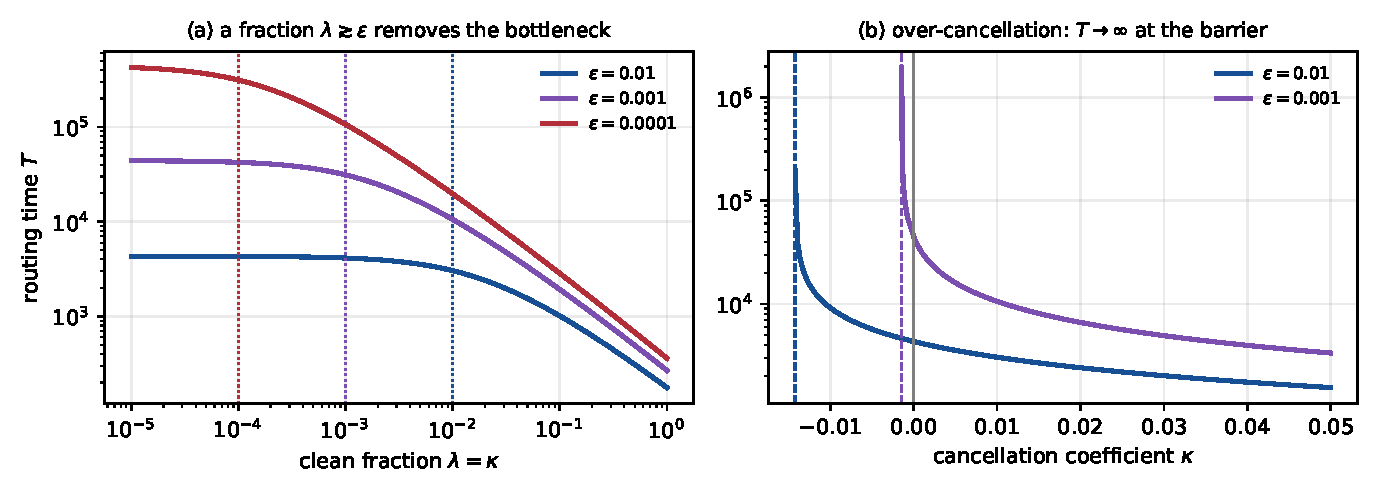
\includegraphics[width=\linewidth]{figures/kappa_sweep.pdf}
\caption{\textbf{Routing time across the cancellation coefficient}, correlation loss, $N=16$, $\eta=0.1$, exact quadrature.
(a) Diluting the anti-copy law with a clean fraction $\lambda=\kappa$: the plateau at $\Theta(\tfrac{1}{\varepsilon})$ ends near $\lambda\approx\varepsilon$ (dotted lines).
(b) Through $\kappa=0$ into over-cancellation: the routing time diverges at the barrier $\varepsilon^2=-F(q_0)$ (dashed lines), at $\kappa\approx-1.4\,\varepsilon$.}
\label{fig:kappa}
\end{figure}

\paragraph{Where the delay accumulates.}
Under $\Dlaw0$, the score gap initially moves at rate $\tfrac{\gamma \varepsilon^2}{N}$ while the leading rule credit is zero.
For small score gaps, $F(q)=\tfrac{q^2}{2}+O(q^3)$, so the rule remains near its initialization until $q$ is of order $\varepsilon$.
Integrating across this neighborhood gives the inverse-initialization delay.
Under $\Dlaw1$, $\left.\dv{F(q)}{q}\right|_{q=0}>0$, and the same integral instead gives a logarithm.
After a fixed positive score gap is reached, the remaining correlation-loss routing time is bounded independently of $\varepsilon$
for fixed $N,\gamma$. This fixed-gap qualification matters: leaving only the interval $q\le \varepsilon$ does not finish the bottleneck.
Under over-cancellation, $\phi<0$ first shrinks the rule; the barrier in $F$ decides whether routing can escape.
The exact threshold, including its equality case, is proved in \cref{thm:separation}(iii). \Cref{fig:phase} shows the three cases in the $(q,r)$ plane.

\begin{figure}[t]
\centering
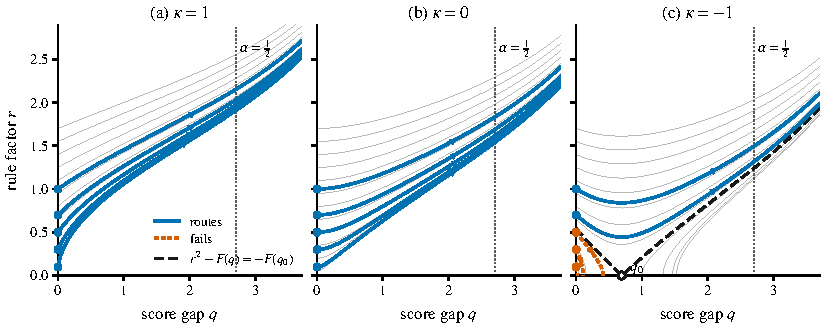
\includegraphics[width=\linewidth]{figures/phase_portrait.pdf}
\caption{\textbf{Phase portrait of the reduced correlation-loss flow.} $N=16$, $\eta=0.1$; grey curves are level sets of the invariant $r^2-F(q)$
(\cref{lem:invariant}), and trajectories start at $(0,\varepsilon)$ for $\varepsilon\in\{0.1,0.3,0.5,0.7,1\}$; the dotted line marks source attention $\alpha=\tfrac12$.
(a)~Under $\Dlaw1$, $F$ is linear near $q=0$ and every trajectory leaves the axis at once; (b)~under $\Dlaw0$, $F(q)=\tfrac{q^2}{2}+O(q^3)$ and small-$\varepsilon$
trajectories creep along it. (c)~Under over-cancellation the rule first shrinks, and the separatrix $r^2-F(q)=-F(q_0)$ through $(q_0,0)$ divides routing from
collapse, the barrier $\varepsilon^2>-F(q_0)$ of \cref{thm:separation}(iii).}
\label{fig:phase}
\end{figure}


The proofs in \cref{app:routing-proof,app:critical} use one attention estimate, one primitive estimate, and the barrier minimum.

% ===================================================================
\section{Cross-entropy: escaping the bottleneck}
\label{sec:crossentropy}
Theorem~\ref{thm:separation}(iv) concerns the escape from uniform attention at fixed $N,\gamma$.
Cross-entropy preserves the matrix reduction and the score metric, but changes the rule gradient.
\begin{proof}[Why the initialization orders persist]
Write $m=r^2$ only in this argument. The exact derivatives in \cref{app:ce-proof} imply,
on a sufficiently small fixed interval $0\le q\le b$ on which $m\le\gamma$,
\[
 m(q)=\Theta(\varepsilon^2+q^{2-\kappa}),\qquad
 \ddt{q}=\Theta(m(q)),\qquad \kappa\in\{0,1\}.
\]
Consequently the local hitting time satisfies
\[
 T(b)=\Theta\!\left(\int_0^b\frac{dq}{\varepsilon^2+q^{2-\kappa}}\right)
 =\begin{cases}
 \Theta(\log(\tfrac{1}{\varepsilon})),&\kappa=1,\\
 \Theta(\tfrac{1}{\varepsilon}),&\kappa=0.
 \end{cases}
\]
The integrating-factor comparison is proved in \cref{app:ce-proof}.
\end{proof}
At finite initialization, cross-entropy initially shrinks the cancelling rule factors at cubic order;
this correction is included in the exact derivative comparison.

\paragraph{Beyond escape.}
For the anti-copy law the attended read takes many values, and at large rule product the cross-entropy score velocity
could in principle change sign before routing. We therefore do not claim complete cross-entropy routing as a theorem.
Numerically it completes in every tested configuration, with the score velocity bounded away from zero along each trajectory,
and the complete-routing times keep the two initialization orders (\cref{tab:network-flow,fig:network-flow}).

% ===================================================================
\section{Full-matrix training: a cross-entropy plateau}
\label{sec:fullmatrix}
\Cref{thm:separation} trains four tied scalars. Could a network whose every matrix entry trains escape the cancellation by learning other features,
other value maps or other attention patterns? Near the structured initialization it cannot. The proof needs no invariant manifold:
it combines the distributional cancellation of \cref{lem:matched} with a loss-floor and energy argument.

\paragraph{The full-matrix network.} Keep the embeddings and type mask of \cref{sec:architecture} fixed, and make every remaining entry trainable:
query and key $Q,K\in\mathbb R^{d\times7}$, value $V\in\mathbb R^{d_v\times7}$, output $O\in\mathbb R^{7\times d_v}$, MLP weights $U\in\mathbb R^{m\times7}$, bias $\bm a\in\mathbb R^m$,
and $D\in\mathbb R^{7\times m}$, and readout $\bm c\in\mathbb R^7$, with $d,d_v\ge1$ and $m\ge4$. The logit is
\[
 z_W=\bm c^\top\bigl[\bm g_b+D\relu(U\bm g_b+\bm a)\bigr],\qquad
 \bm g_b=\bm h_q^{(0)}+O\sum_{j=1}^N\alpha_jV\bm h_j^{(0)},\qquad
 \bm\alpha=\softmax\bigl((Q\bm h_q^{(0)})^\top K\bm h_j^{(0)}\bigr)_j .
\]
Let $W_0$ be the matrices of \cref{eq:attention-matrices,eq:mlp-matrices} at $\bm\theta(0)$, padded with zeros, with readout $\bm c=\bm e_7$; nothing is tied afterwards.
Training follows $\dot W\in-\partial\mathcal L_{\mathrm{ce}}(W)$, the Clarke subgradient flow, which is ordinary gradient flow wherever the loss is differentiable.

\begin{mainresult}
\begin{theorem}[Full-matrix cross-entropy plateau]
\label{thm:fullmatrix}
Under $\Dlaw0$, let $B\ge1$, $C_B=110(B+2)$ and $0<\varepsilon\le\tfrac{1}{10}$.
\begin{enumerate}[label=(\roman*),leftmargin=*,itemsep=2pt,topsep=2pt]
\item \emph{Weak credit near initialization.} Every $W$ with $\|W-W_0\|_F\le\varepsilon$ has
$|\E[Yz_W]|\le\gamma C_B\varepsilon^3$ and therefore $\mathcal L_{\mathrm{ce}}(W)\ge\log2-\tfrac12\gamma C_B\varepsilon^3$.
\item \emph{Plateau.} From $W(0)=W_0$, for all $0\le t<\tfrac{1}{C_B\varepsilon}$,
\[
 \|W(t)-W_0\|_F<\varepsilon,\qquad \mathcal L_{\mathrm{ce}}(W(t))\ge\log2-\tfrac12\gamma C_B\varepsilon^3 .
\]
Reaching any loss below $\log2-\delta$ with $\delta>\tfrac12\gamma C_B\varepsilon^3$ therefore takes time at least $\tfrac{1}{C_B\varepsilon}$.
\item \emph{Perturbed starts.} There is $L_B$ depending only on $B$ such that the same holds, with exit time at least $\tfrac{1}{4(C_B+(1+L_B)^2)\varepsilon}$,
from every $W(0)$ with $\|W(0)-W_0\|_F\le\varepsilon^{3/2}$.
\end{enumerate}
\end{theorem}
\end{mainresult}

\paragraph{Why the plateau holds.} At uniform attention the network sees only the instruction and the average embedding, which under $\Dlaw0$ is independent of the source, so
its logit has zero correlation with the label, whatever its other weights are (\cref{lem:matched}). Near $W_0$ attention can depart from uniform only by $O(\varepsilon)$,
and its dependence on the instruction, which the label needs, only by $O(\varepsilon^2)$: the key starts at zero and the query does not read the instruction.
Every path from attention to the logit passes through a product that starts at zero or at $O(\varepsilon)$, giving $|\E[Yz_W]|=O(\varepsilon^3)$.
Cross-entropy equals $\log2-\tfrac12\E[Yz]+\E\log\cosh\tfrac{z}{2}$, so the loss cannot fall by more than $O(\varepsilon^3)$ inside the ball, and the energy identity
$\|W(t)-W_0\|_F^2\le t\,[\mathcal L(W_0)-\mathcal L(W(t))]$ turns that into an exit time of order $\tfrac{1}{\varepsilon}$ (\cref{app:fullmatrix}).

\paragraph{What it does not say.} The theorem is a lower bound for the cancelled law only. It does not give the exact $\Theta(\tfrac{N}{\varepsilon})$ routing time,
the conserved quantity or the failure barrier for full matrices, and it does not prove that the independent law escapes fast; the
experiments in \cref{sec:numerics} compare the two. It covers the structured start and perturbations of size $\varepsilon^{3/2}$, not perturbations of fixed size
or fully random initialization. A loss near $\log2$ also does not by itself mean chance accuracy.

% ===================================================================
\section{Causal corrupted reasoning traces}
\label{sec:causal}
The anti-copy laws also separate when $\eta=0$: there the mechanism is contextual correlation, rather than incorrect labels.
We now keep the instruction process fixed and make the error process itself create the correlations.
The same block is trained jointly on $N$ consecutive next-state predictions, each with local error rate $\eta>0$.

\paragraph{Construction.}
Fix $\eta\in(0,\tfrac{1}{2})$, $\gamma=1-2\eta$, and $N\ge4$ such that
\[
 \frac{2}{N-1}<\min\{2\eta,\gamma\}.
\]
Start from $x_1=\cdots=x_N=w$, with $w$ uniform and $b_2=\cdots=b_N=1$.
For $i=N,\ldots,2N$, draw a fresh uniform $b_{i+1}$ and set $x_{i+1}=b_{i+1}x_i \xi_{i+1}$.
The two error regimes are
\begin{align}
 \text{independent:}\quad&\Pr(\xi_{i+1}=-1\mid\bm x_{<i+1},b_{i+1})=\eta,\notag\\
 \text{cancelling:}\quad&\Pr(\xi_{i+1}=-1\mid\bm x_{<i+1},b_{i+1})
 =\eta+\frac{b_{i+1}x_i\sum_{j=1}^i x_j}{2(N^2+N-i)}.
 \label{eq:causal-kernel}
\end{align}
Supervise every position $i=N+1,\ldots,2N$ with target $x_{i+1}$.
A fully correct control uses the same seed, instructions and supervised positions with $\xi_{i+1}=1$ at every step.

\begin{mainresult}\begin{theorem}[Wrong CoT steps generate credit cancellation]
\label{thm:causal}
For the construction above, compare the independent and cancelling error regimes.
Both regimes have uniform displayed-state marginals and, at every supervised position,
\[
 \Pr(x_{i+1}\ne b_{i+1}x_i\mid x_i,b_{i+1})=\eta,
 \qquad \hat x_{i+1}=b_{i+1}x_i
\]
as the Bayes predictor even given the full prefix.
Their cancellation coefficients are respectively
\[
 1+\sum_{j<i}\E[x_i x_j]=1\qquad\text{and}\qquad
 1+\sum_{j<i}\E[x_i x_j]=0.
\]
The complete trace has $2N$ transitions and expected incorrect fraction
$\tfrac{\eta(N+1)}{2N}\to\tfrac{\eta}{2}>0$.
More strongly, the number of incorrect transitions satisfies
\[
 N_{\mathrm w}\sim\operatorname{Binomial}(N+1,\eta),\qquad
 \Pr\!\left(\frac{N_{\mathrm w}}{2N}\ge\frac{\eta}{4}\right)
 \ge1-\exp\!\left(-\frac{\eta(N+1)}{8}\right).
\]
Train the same four coordinates from \cref{eq:initialization}, averaging correlation loss over these $N$ supervised prefixes.
Use the last visible state as source in each prefix and fix $B>\sqrt{\varepsilon^2+3\log(2N-1)}$ before training.
Let $T$ be the first time every supervised prefix has source attention at least $\tfrac{1}{2}$.
For $0<\varepsilon\le1$,
\begin{align*}
 T_{\mathrm{clean}}&=\Theta(N\log(1+\varepsilon^{-2})),&
 T_{\mathrm{independent}}&=\frac{T_{\mathrm{clean}}}{\gamma},\\
 T_{\mathrm{cancelling}}&=\Theta\!\left(\frac{N}{\gamma\varepsilon}\right).
\end{align*}
with absolute comparison constants. All three regimes reach the correct Bayes computation on a gate-valid interval beyond routing.
For fixed admissible $N,\eta$ and sufficiently small $\varepsilon$, $T_{\mathrm{cancelling}}>T_{\mathrm{independent}}>T_{\mathrm{clean}}$.
\end{theorem}\end{mainresult}
The cancelling kernel is a balancing bias. Its correction is proportional to $b_{i+1}x_i S_i$, the correct next state times the running sum of
displayed states, so a slip is slightly more likely when the correct step would extend the majority, and wrong steps keep the history balanced.
Exact balance is not required for the delay: within the anti-copy family, \cref{cor:dilution} keeps the order $\tfrac{1}{\varepsilon}$ for every
$\kappa\in[0,c\varepsilon]$.
\Needspace{0.35\textheight}
\begin{proof}[The cancellation mechanism]
Write $S_i=\sum_{j=1}^i x_j$ and $V_i=N^2+N-i$ for this calculation.
Averaging the fresh uniform instruction in the cancelling kernel gives
\[
 \E[x_{i+1}\mid\bm x_{<i+1}]=-\frac{S_i}{V_i}.
\]
At the seed, $\E[S_N^2]=N^2=V_N$. Inductively,
\begin{align*}
 \E[x_{i+1}S_i]&=-\frac{\E[S_i^2]}{V_i}=-1,\\
 \E[S_{i+1}^2]&=\E[S_i^2]+2\E[x_{i+1}S_i]+1=V_i-1=V_{i+1},\\
 \E[x_{i+1}S_{i+1}]&=\E[x_{i+1}S_i]+1=0.
\end{align*}
Hence $1+\sum_{j<i+1}\E[x_{i+1}x_j]=0$ at every selected prediction position.
With independent errors, each fresh instruction instead makes $x_{i+1}$ independent of its displayed past,
giving coefficient $1$.
The probability bounds, matched local laws, binomial error count and shared-parameter routing comparison are proved in \cref{app:trace-proof}.
\end{proof}
The errors are history dependent in the cancelling regime; the instructions have the same fresh-uniform law in both.
The condition on $N$ is essential for the cancelling regime: it cannot be satisfied at $\eta=0$.
Its coefficient is $\kappa=0$ for every admissible positive $\eta$; the construction does not assert a continuous interpolation $\kappa(\eta)$ from the clean regime.
Its cancellation holds in conditional mean, $\E[S_i\mid x_i]=0$ at every supervised position (\cref{app:trace-proof}), which is what the tied block reads.
It is weaker than the full independence of \cref{lem:matched}; a causal error process with distributional cancellation is left open.

% ===================================================================
\section{Experiments matched to the claims}
\label{sec:numerics}

\paragraph{Does the network produce the derived gradients?}
We first instantiate the matrices and residual paths of \cref{sec:architecture}, rather than directly coding its reduced logit.
Across 72 configurations spanning three context sizes, four cancellation coefficients, two losses, and three score/weight settings,
autograd agrees with the analytical logits and velocities to absolute tolerance $10^{-12}$.
This checks both the neural realization and the factor of two arising from the two trainable score groups.
All supported prefixes and errors are enumerated with their exact masses, so there is no sampling variability (\cref{app:network-experiments}).

\paragraph{Matched loss comparison.}
\Cref{tab:network-flow} reports continuous gradient-flow times at error probability $0.1$.
The initialization, context size, population law, stopping rule and parameter metric are held fixed between the two losses.
The correlation runs test \cref{thm:separation}(i)--(ii); the cross-entropy runs test the escape orders of \cref{thm:separation}(iv)
and the complete routing that we verify only numerically.
\Cref{fig:network-flow} separately displays escape to score gap $0.01$ and routing to source attention $\tfrac{1}{2}$.

\begin{table}[t]
\centering\small
\caption{\textbf{Matched population-flow experiment in the derived one-block parameterization.}
Error probability $\eta=0.1$. Subscripts $1$ and $0$ denote the independent law $\Dlaw1$ and the anti-copy law $\Dlaw0$.
All columns are continuous gradient-flow time.}
\label{tab:network-flow}
\begin{tabular}{@{}rr rrrr@{}}
\toprule
$N$ & $\varepsilon$ & $T_{\mathrm{corr},1}$ & $T_{\mathrm{corr},0}$ & $T_{\mathrm{ce},1}$ & $T_{\mathrm{ce},0}$\\
\midrule
16 & 0.03 & 133.1 & 1,380.0 & 140.9 & 1,406.8\\
16 & 0.01 & 176.9 & 4,316.4 & 184.8 & 4,351.2\\
16 & 0.003 & 225.0 & 14,655.1 & 232.9 & 14,698.7\\
16 & 0.001 & 269.0 & 44,248.7 & 276.9 & 44,300.3\\
64 & 0.03 & 520.6 & 5,480.0 & 546.4 & 5,593.7\\
64 & 0.01 & 695.9 & 17,214.8 & 721.7 & 17,363.5\\
64 & 0.003 & 888.5 & 58,557.6 & 914.3 & 58,745.0\\
64 & 0.001 & 1,064.3 & 176,921.0 & 1,090.1 & 177,143.8\\
\bottomrule
\end{tabular}

\end{table}
\begin{figure}[t]
\centering
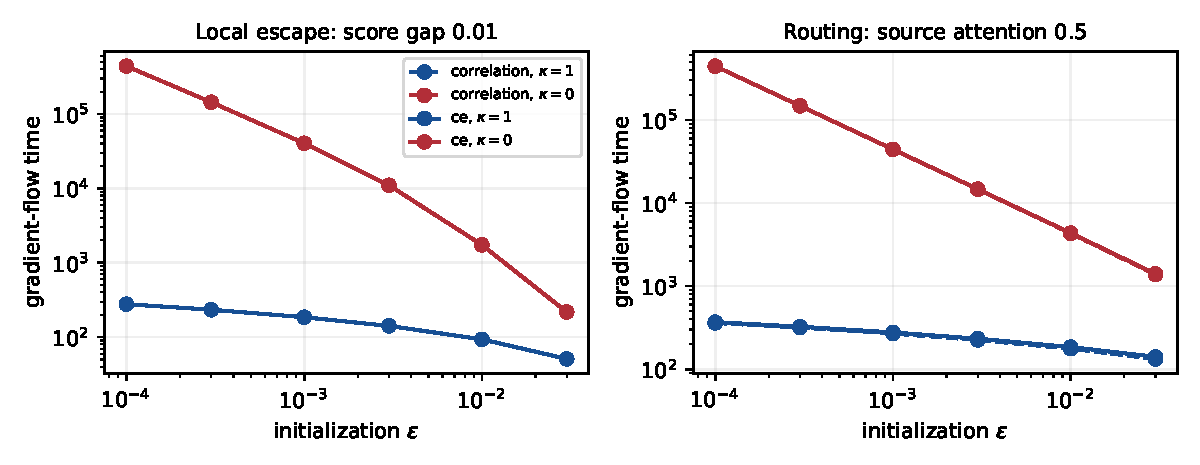
\includegraphics[width=\linewidth]{figures/one_block_scaling.pdf}
\caption{\textbf{Separate tests of escape and full routing.} Context size $N=16$, error probability $\eta=0.1$.
Dashed curves use correlation loss and solid curves use cross-entropy, with otherwise matched settings.
The theorem predicts distinct initialization orders for both local escape and complete routing.}
\label{fig:network-flow}
\end{figure}

\paragraph{The exact quadrature.} Direct integration of the flow of \cref{lem:invariant} agrees with \cref{eq:time} to five significant
figures, and the conserved quantity drifts by at most $6\times10^{-9}$, for $N\in\{16,64,256\}$ and $\varepsilon\in\{10^{-2},10^{-3}\}$;
every bound of \cref{thm:separation} holds (\cref{tab:quadrature}). Over-cancellation follows the exact criterion of
\cref{thm:separation}(iii): at $N=64$ and $\varepsilon=0.01$, routing completes at $\kappa=-0.007$, where $-F(q_0)<\varepsilon^2$, and does not
complete at $\kappa=-0.0283$, where $-F(q_0)\simeq3.9\times10^{-4}>\varepsilon^2$. The routing time is linear in $N$ under both laws. Reducing
$\varepsilon$ tenfold multiplies $\Tr(\Dlaw0)$ by $10.3$ and $\Tr(\Dlaw1)$ by $1.5$.

\paragraph{Diluting the cancellation.} \texttt{kappa\_sweep.py} integrates the primitive and the routing time together for $\kappa\in[-1,1]$ (\cref{fig:kappa}).
For clean fractions $\lambda\in[0,1]$, $N\in\{16,64\}$ and $\varepsilon\in\{10^{-2},10^{-3},10^{-4}\}$, the exact routing time stays within a factor $1.03$--$1.51$ of
$\tfrac{N-1}{\gamma}\int_0^1\tfrac{dq}{\varepsilon^2+\lambda q+q^2}$, the quantity that \cref{cor:dilution} evaluates. At $N=16$ the over-cancellation barrier sits at
$\kappa=-0.0142$ for $\varepsilon=10^{-2}$ and at $\kappa=-0.00141$ for $\varepsilon=10^{-3}$.

\begin{table}[t]
\caption{\textbf{Exact routing times of the correlation-loss flow.} $\gamma=1$. ODE: direct integration; quadrature: \cref{eq:time}; drift:
largest deviation of $r^2-F(q)-\varepsilon^2$ along the trajectory.}
\label{tab:quadrature}
\centering\small
\begin{tabular}{@{}rr rr rr r@{}}
\toprule
 & & \multicolumn{2}{c}{$\Dlaw1$} & \multicolumn{2}{c}{$\Dlaw0$} & \\
\cmidrule(lr){3-4}\cmidrule(lr){5-6}
$N$ & $\varepsilon$ & ODE & quadrature & ODE & quadrature & ratio\\
\midrule
16  & $10^{-2}$ & 141.5  & 141.5  & 3{,}453   & 3{,}453   & 24\\
16  & $10^{-3}$ & 215.2  & 215.2  & 35{,}399  & 35{,}399  & 164\\
64  & $10^{-2}$ & 556.8  & 556.8  & 13{,}772  & 13{,}772  & 25\\
64  & $10^{-3}$ & 851.4  & 851.4  & 141{,}540 & 141{,}540 & 166\\
256 & $10^{-2}$ & 2{,}215 & 2{,}215 & 55{,}043  & 55{,}043  & 25\\
256 & $10^{-3}$ & 3{,}394 & 3{,}394 & 566{,}080 & 566{,}080 & 167\\
\bottomrule
\end{tabular}
\end{table}

\paragraph{Does the causal error process match the new theorem?}
\texttt{causal\_credit.py} propagates the exact finite-state law of the prefix sum and final sign.
For $\eta=0.2$ and $N\in\{8,16,32\}$, it checks every supervised position's local error rate, cancellation coefficient, and the cancelling variance recurrence.
Propagating the error count jointly with these states also verifies the binomial law and the high-probability bound.
An additional 18 matrix-gradient configurations enumerate both instructions and both error signs under the history-dependent kernel.
The largest gradient discrepancy is below $10^{-12}$; there is no Monte Carlo estimation.
\Cref{tab:causal-flow} reports 36 averaged-loss routing runs across fully correct, independently corrupted and structured corrupted supervision.
All three share the initialization, seed and instruction process; the two noisy regimes share $\eta=0.2$.
Nine further matrix configurations verify the fully correct control.
The independent-noise times agree with $T_{\mathrm{clean}}/(1-2\eta)$ to relative error below $10^{-10}$.
The expected incorrect fraction is $0.1125$, $0.10625$, and $0.103125$ for $N=8,16,32$, respectively, approaching $0.1$.
For $N=16$, reducing $\varepsilon$ from $0.01$ to $0.001$ increases routing time by a factor $1.52$ with independent errors and $10.26$ with cancelling errors.
All runs satisfy the explicit bounds in \cref{app:trace-proof}.
At $N=16$ and $\varepsilon=0.01$, eight additional runs sweep $\eta\in\{0.1,0.2,0.3,0.4\}$ in the two noisy regimes.
The rescaled times $(1-2\eta)T$ remain constant to relative error below $10^{-10}$: about $207.9$ for independent errors and $5{,}089.6$ for structured errors.

\begin{table}[t]
\centering\small
\caption{\textbf{Correct computation from clean and corrupted reasoning supervision.} The clean control has no errors; both noisy regimes have local error rate $\eta=0.2$.
The same block parameters train on all $N$ selected positions. Times reach source attention $\tfrac{1}{2}$ on every prefix; the final column compares structured errors with clean supervision.}
\label{tab:causal-flow}
\begin{tabular}{@{}rr rrrr@{}}
\toprule
$N$ & $\varepsilon$ & clean & independent & structured & ratio to clean\\
\midrule
8 & 0.03 & 81.3 & 135.6 & 1,393.2 & 17.1\\
8 & 0.01 & 107.8 & 179.7 & 4,347.9 & 40.3\\
8 & 0.003 & 136.8 & 228.1 & 14,747.2 & 107.8\\
8 & 0.001 & 163.4 & 272.3 & 44,511.6 & 272.5\\
16 & 0.03 & 156.1 & 260.2 & 2,708.0 & 17.3\\
16 & 0.01 & 207.9 & 346.5 & 8,482.6 & 40.8\\
16 & 0.003 & 264.7 & 441.2 & 28,819.0 & 108.9\\
16 & 0.001 & 316.6 & 527.6 & 87,034.8 & 274.9\\
32 & 0.03 & 305.2 & 508.7 & 5,336.7 & 17.5\\
32 & 0.01 & 407.5 & 679.2 & 16,752.4 & 41.1\\
32 & 0.003 & 519.9 & 866.5 & 56,967.0 & 109.6\\
32 & 0.001 & 622.5 & 1,037.5 & 172,097.6 & 276.5\\
\bottomrule
\end{tabular}

\end{table}

\paragraph{Does the separation survive untying?}
We next train every entry of the one-block network independently: all seven-by-seven query, key, value and output matrices,
both MLP layers with their bias, and the readout, under binary cross-entropy on the exact population of $\Dlaw\kappa$, $N=16$, $\eta=0.1$.
Three initialization families move progressively away from the theorem.
(A) The directions of \cref{sec:architecture} with random magnitudes: fixed directions get magnitudes in $[\tfrac{1}{2},2]$,
each of the eight MLP rule entries gets $\varepsilon$ times a magnitude in $[\tfrac{1}{2},2]$, with a random sign per layer, and the four MLP units are no longer tied.
(B) The same plus independent Gaussian noise of fan-in scale $0.1$ or $0.3$ on every matrix.
(C) Fan-in Gaussian matrices scaled by $\varepsilon$, a sixteen-unit MLP, and nothing hand-coded.
Full-batch gradient descent with backtracking measures time on the gradient-flow clock (\cref{app:network-experiments}).

\Cref{tab:untied} reports how many of three seeds reach $99\%$ clean-rule accuracy within flow time $3\times10^4$.
With clean supervision, every seed of family (B) learns at every $\varepsilon\le0.1$, within $51$ time units,
and two of three seeds of family (A) learn at every $\varepsilon\le0.5$; the third starts with opposite rule-factor signs in the two MLP layers and fails at every $\varepsilon$.
Exact cancellation stalls: with noise, no seed learns below $\varepsilon=0.1$ ($0.1$ noise) or $\varepsilon=0.5$ ($0.3$ noise);
without noise, the seeds that learn slow down roughly as $\tfrac{1}{\varepsilon}$, from $24$ time units at $\varepsilon=0.3$ to $2{,}514$ at $\varepsilon=0.003$.
Over-cancellation fails at every $\varepsilon\le0.3$ and recovers only at $\varepsilon\ge0.5$ ($\varepsilon=1$ with $0.3$ noise),
the untied counterpart of the barrier in \cref{thm:separation}(iii).
In family (C), with three seeds and gradient descent, the three laws do not separate clearly; the next paragraph tests this regime at scale.

\paragraph{Does the full-matrix plateau appear?}
\texttt{full\_matrix\_plateau.py} trains every entry from exactly $W_0$, $N=16$, $\eta=0.1$, by gradient descent with step $0.5$, and records the first flow time at which
$\|W-W_0\|_F=\varepsilon$. Under the anti-copy law the exit time is $1{,}048$, $1{,}579$, $3{,}170$, $6{,}351$, $10{,}592$ and $15{,}893$ for
$\varepsilon=0.03,0.02,0.01,0.005,0.003,0.002$, that is between $31.4/\varepsilon$ and $31.8/\varepsilon$, and the largest $|\E[Yz_W]|$ inside the ball is $0.065\,\varepsilon^3$ at every $\varepsilon$:
the order of \cref{thm:fullmatrix}, with a much smaller constant than the proved $\gamma C_B=528$. Under the independent law every run leaves the ball at flow time $23$,
whatever $\varepsilon$ is, and its correlation inside the ball scales as $\varepsilon^2$. The full-matrix network can therefore escape quickly when credit is not cancelled.

\paragraph{From fully random initialization.}
We repeat family (C) with ten seeds, $N\in\{8,16,32\}$, $\varepsilon\in\{0.05,0.1,0.2,0.3,0.5,0.7,1,1.5\}$, and two optimizers: backtracking gradient descent with
flow-time budget $10^5$, and Adam with step size $3\times10^{-3}$ for $10^5$ steps (\cref{tab:randinit}).
The first escape from chance takes the same time under every law (for Adam, a median of $45$, $52$ and $60$ steps at $N=8,16,32$, within a few steps across $\kappa$):
from random matrices it is limited by the product of small weights, not by the data, as in deep linear networks.
The laws differ in where training goes next. With Adam, all $240$ runs on the independent law reach the Bayes predictor; on the anti-copy law $33$--$40\%$ of runs
stall, and with two anti-copies $43$--$50\%$. All $195$ stalled runs are flat, with loss changing by less than $10^{-4}$ over the last $4\times10^4$ steps, and $193$ of them sit at a single stationary point
for each law and context size, with loss $0.43$--$0.50$ against the Bayes value $0.325$ and clean accuracy $79$--$91\%$. Gradient descent shows the same ordering among initializations $\varepsilon\ge0.5$, where the
independent law learns reliably. From random initialization, then, cancellation does not delay the first escape; it makes training land in a worse stationary point.

\begin{table}[t]
\centering\small
\caption{\textbf{Fully random initialization, every matrix entry trained.} Anti-copy law, $\eta=0.1$, binary cross-entropy, ten seeds per initialization.
Each cell: runs reaching $99\%$ clean-rule accuracy within the budget; Adam pools eight initializations, gradient descent the four with $\varepsilon\ge0.5$.}
\label{tab:randinit}
\begin{tabular}{@{}lcccccc@{}}
\toprule
 & \multicolumn{3}{c}{Adam, all $\varepsilon$} & \multicolumn{3}{c}{GD, $\varepsilon\ge0.5$}\\
\cmidrule(lr){2-4}\cmidrule(lr){5-7}
$N$ & $\kappa=1$ & $\kappa=0$ & $\kappa=-1$ & $\kappa=1$ & $\kappa=0$ & $\kappa=-1$\\
\midrule
8 & 80/80 & 54/80 & 45/80 & 37/40 & 24/40 & 20/40\\
16 & 80/80 & 52/80 & 46/80 & 34/40 & 23/40 & 19/40\\
32 & 80/80 & 48/80 & 40/80 & 33/40 & 23/40 & 19/40\\
\bottomrule
\end{tabular}

\end{table}

\begin{table}[t]
\centering\small
\caption{\textbf{Untied one-block training under the anti-copy law.} Every matrix entry trains; binary cross-entropy, $N=16$, $\eta=0.1$.
Each cell: seeds (of three) reaching $99\%$ clean-rule accuracy within gradient-flow time $3\times10^4$, and their median time.
$\kappa=1$: independent decoys; $\kappa=0$: one anti-copy; $\kappa=-1$: two anti-copies.}
\label{tab:untied}
\fitwidth{\begin{tabular}{@{}llcccccc@{}}
\toprule
Initialization & $\kappa$ & $\varepsilon=0.003$ & $\varepsilon=0.03$ & $\varepsilon=0.1$ & $\varepsilon=0.3$ & $\varepsilon=0.5$ & $\varepsilon=1$\\
\midrule
A: directions & $+1$ & 2/3 (85) & 2/3 (59) & 2/3 (34) & 2/3 (14) & 2/3 (9) & 1/3 (4)\\
 & $+0$ & 1/3 (2,514) & 2/3 (497) & 2/3 (114) & 2/3 (24) & 1/3 (9) & 1/3 (4)\\
 & $-1$ & 0/3 & 0/3 & 0/3 & 0/3 & 1/3 (26) & 1/3 (4)\\
\addlinespace
B: $+\,0.1$ noise & $+1$ & 3/3 (51) & 3/3 (44) & 3/3 (34) & 2/3 (14) & 2/3 (8) & 2/3 (57)\\
 & $+0$ & 0/3 & 0/3 & 1/3 (97) & 1/3 (20) & 1/3 (10) & 1/3 (4)\\
 & $-1$ & 0/3 & 0/3 & 0/3 & 0/3 & 2/3 (454) & 1/3 (5)\\
\addlinespace
B: $+\,0.3$ noise & $+1$ & 3/3 (34) & 3/3 (34) & 3/3 (30) & 3/3 (20) & 3/3 (11) & 2/3 (19)\\
 & $+0$ & 0/3 & 0/3 & 0/3 & 0/3 & 1/3 (20) & 1/3 (6)\\
 & $-1$ & 0/3 & 0/3 & 0/3 & 0/3 & 0/3 & 1/3 (11)\\
\addlinespace
C: random & $+1$ & 0/3 & 0/3 & 1/3 (26,330) & 1/3 (1,009) & 2/3 (168) & 3/3 (44)\\
 & $+0$ & 0/3 & 0/3 & 1/3 (23,109) & 1/3 (885) & 1/3 (211) & 2/3 (21)\\
 & $-1$ & 0/3 & 0/3 & 1/3 (23,109) & 1/3 (885) & 1/3 (185) & 2/3 (22)\\
\bottomrule
\end{tabular}
}
\end{table}

% ===================================================================
\section{Discussion and limitations}
\label{sec:scope}
The model supplies the value direction, instruction interaction and relative source indicator; it learns routing and both rule factors.
The causal theorem trains all $N$ prediction examples after a supplied seed and one warm-up transition.
It gives a constant fraction of incorrect transitions with high probability, while leaving the seed transitions unsupervised; the process is nonstationary.
Each prefix is encoded with the source flag at its last visible state, and the same four parameters are shared across prefixes.
The matched laws have the same local error rate and Bayes predictor; their conditional error probabilities given the complete prefix can differ.
The exact reliability rescaling is a correlation-loss statement, and complete cross-entropy routing under the anti-copy law is verified numerically, not proved.
In the causal cancelling regime, $\eta$ varies only within the admissible range;
we do not infer cancellation from the noise percentage alone or extend the construction continuously to $\eta=0$.
The delay in time is proved near the structured initialization (\cref{thm:fullmatrix}) and observed when training starts from the specified directions;
from fully random initialization the first escape is depth-limited and law-independent, and cancellation shows up as a higher rate of stalling instead.
We do not yet characterize the stalled stationary point or prove that the independent law escapes fast in full-matrix training.

% ===================================================================
\paragraph{Relation to prior work.}
\label{sec:related}

Corrupted chains of thought have been studied with static and propagated noise \citep{havrilla2024noise}
and noisy rationales at inference \citep{zhou2024noisyrationales}. Classical label-noise conditions
\citep{natarajan2013noisy,patrini2017loss} address statistical recovery; our matched laws differ in optimization.
Scratchpads and process supervision \citep{nye2021scratchpads,wei2022cot,uesato2022solving,lightman2023verify}
have been analysed through statistical rates \citep{jia2025verify,hanneke2026samplecomplexityautoregressivereasoning},
sparse dependence \citep{wen2024sparse}, and parity learning \citep{kim2024parity}.
We fix the supervision format and study its error structure.
Weak-gradient \citep{shalevshwartz2017failures,abbe2025parities} and leap-based SGD analyses
\citep{abbe2021staircase,abbe2023sgd} relate slow learning to weak target correlation.
Here the source--target correlation is fixed, while the sum over attended positions cancels.
The resulting delay resembles small-initialization saddle escape in deep linear networks
\citep{saxe2014exact,shamir2019exponential}, with the saddle induced by the data correlations.

% ===================================================================
\paragraph{Implications.}
\label{sec:conclusion}

Correct reasoning can survive incorrect chain-of-thought supervision, but learning time depends on how errors interact with attention:
independent errors weaken useful credit, while structured errors can cancel it and create an inverse-initialization bottleneck.
For the bottleneck to bind a network that is free to compute other features, the cancellation must be distributional, as for a single anti-copy step.
Extending these results to random initialization, to causal processes with distributional cancellation, and to training every position without a supplied seed remains open.
